\documentclass[12pt,aspectratio=169]{beamer}
\usepackage{amsmath, amssymb}
\usepackage{booktabs}
\usepackage{tikz}
\usetikzlibrary{arrows.meta,decorations.pathmorphing,patterns,calc}
\usepackage{xcolor}
\usepackage{array}
\usepackage{chemformula}

% -- Theme (identical to all previous decks) ---------------------------
\usetheme{Madrid}
\definecolor{firered}{RGB}{180,30,10}
\definecolor{ashgrey}{RGB}{50,55,65}
\definecolor{skyblue}{RGB}{30,100,180}
\definecolor{flameyellow}{RGB}{230,155,15}
\setbeamercolor{palette primary}{bg=ashgrey,fg=white}
\setbeamercolor{palette secondary}{bg=ashgrey!85,fg=white}
\setbeamercolor{palette tertiary}{bg=ashgrey!65,fg=white}
\setbeamercolor{palette quaternary}{bg=ashgrey,fg=white}
\setbeamercolor{structure}{fg=skyblue}
\setbeamercolor{alerted text}{fg=firered}
\setbeamercolor{block title}{bg=skyblue,fg=white}
\setbeamercolor{block body}{bg=skyblue!8}
\setbeamercolor{block title alerted}{bg=firered,fg=white}
\setbeamercolor{block body alerted}{bg=firered!10}
\setbeamercolor{block title example}{bg=ashgrey,fg=white}
\setbeamercolor{block body example}{bg=ashgrey!10}
\setbeamerfont{title}{size=\Large,series=\bfseries}
\setbeamertemplate{navigation symbols}{}
\setlength{\itemsep}{1pt}

% -- Macros ------------------------------------------------------------
\newcommand{\Da}{\mathrm{Da}}
\newcommand{\Le}{\mathrm{Le}}
\newcommand{\Rey}{\mathrm{Re}}
\newcommand{\ddx}[1]{\frac{d#1}{dx}}
\newcommand{\pd}[2]{\frac{\partial #1}{\partial #2}}
\newcommand{\Tst}{T_{\text{st}}}
\newcommand{\Yf}{Y_F}
\newcommand{\Yox}{Y_{\text{ox}}}
\newcommand{\Zst}{Z_{\text{st}}}
\newcommand{\wdot}{\dot{\omega}}
\newcommand{\chist}{\chi_{\text{st}}}
\newcommand{\chiext}{\chi_{\text{ext}}}
\newcommand{\mdot}{\dot{m}}
\newcommand{\SL}{S_L}
\newcommand{\tchem}{t_{\text{chem}}}
\newcommand{\Tad}{T_{\text{ad}}}
\newcommand{\taures}{\tau}
\newcommand{\Ma}{\mathrm{Ma}}
\newcommand{\code}[1]{\texttt{#1}}
\newcommand{\Lf}{L_f}

% =====================================================================
\title{Diffusion Flames}
\subtitle{Non-Premixed Combustion: Structure, Scaling, and Aero Applications}
\author{Prof.Dr. Onur Tuncer}
\institute{ITU Dept. of Aeronautical Eng.}
\date{\today}

\begin{document}

\begin{frame}
  \titlepage
\end{frame}

\begin{frame}{Lecture Outline}
  \tableofcontents
\end{frame}

% =====================================================================
\section{What is a Diffusion Flame?}
% =====================================================================

\begin{frame}{The Defining Characteristic: Mixing Controls Burning}

  \begin{columns}
    \begin{column}{0.50\textwidth}
      In a \textbf{diffusion (non-premixed) flame}:
      \begin{itemize}
        \item Fuel and oxidiser are \emph{initially separated}
        \item They meet at the reaction zone solely by \textbf{diffusion}
        \item The flame sits at the \textbf{stoichiometric surface}
              where fuel and oxidiser arrive in stoichiometric ratio
        \item Burn rate is set by the \emph{mixing rate}, not kinetics
      \end{itemize}
      \vspace{4pt}
      \begin{block}{Consequence}
        There is no propagation speed, no flammability limit,
        and no risk of flashback --- but soot, NO$_x$,
        and incomplete combustion are harder to control.
      \end{block}
    \end{column}
    \begin{column}{0.46\textwidth}
      \centering
      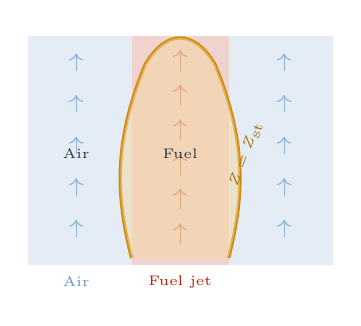
\begin{tikzpicture}[font=\small, scale=0.88]
        % Fuel jet (centre)
        \fill[firered!20] (-0.7,-0.1) rectangle (0.7,3.2);
        \foreach \y in {0.2,0.7,1.2,1.7,2.2,2.7}{
          \draw[->,firered!60,thin] (0,\y)--(0,\y+0.3);
        }
        \node[firered,font=\tiny] at (0,-0.35) {Fuel jet};

        % Coflow air (outer)
        \fill[skyblue!12] (-2.2,-0.1) rectangle (-0.7,3.2);
        \fill[skyblue!12] ( 0.7,-0.1) rectangle ( 2.2,3.2);
        \foreach \y in {0.3,0.9,1.5,2.1,2.7}{
          \draw[->,skyblue!50,thin] (-1.5,\y)--(-1.5,\y+0.25);
          \draw[->,skyblue!50,thin] ( 1.5,\y)--( 1.5,\y+0.25);
        }
        \node[skyblue!70,font=\tiny] at (-1.5,-0.35) {Air};

        % Flame surface (stoichiometric)
        \draw[flameyellow!90!black, very thick]
          (-0.7,0)
          .. controls (-0.9,0.8) and (-1.0,1.6) ..
          (-0.5,2.8)
          .. controls (-0.2,3.3) and (0.2,3.3) ..
          (0.5,2.8)
          .. controls (1.0,1.6) and (0.9,0.8) ..
          (0.7,0);
        \fill[flameyellow!40,opacity=0.5]
          (-0.7,0)
          .. controls (-0.9,0.8) and (-1.0,1.6) ..
          (-0.5,2.8)
          .. controls (-0.2,3.3) and (0.2,3.3) ..
          (0.5,2.8)
          .. controls (1.0,1.6) and (0.9,0.8) ..
          (0.7,0) -- cycle;

        % Label
        \node[flameyellow!70!black,font=\tiny,rotate=70]
          at (0.95,1.5) {$Z = \Zst$};
        \node[font=\tiny,ashgrey] at (0,1.5) {Fuel};
        \node[font=\tiny,ashgrey] at (-1.5,1.5) {Air};
      \end{tikzpicture}
    \end{column}
  \end{columns}
\end{frame}

\begin{frame}{Diffusion Flames in Aerospace Propulsion}

  \begin{center}
  \renewcommand{\arraystretch}{1.35}
  \begin{tabular}{>{\bfseries}p{3.2cm} p{4.0cm} p{4.8cm}}
    \toprule
    System & Configuration & Diffusion-flame role \\
    \midrule
    Gas turbine (conventional) & Jet-A spray into swirl-stabilised
      primary zone & Rich-burn zone is a turbulent diffusion flame
      around evaporating droplets \\
    RQL combustor & Rich primary + quench + lean burn &
      Primary zone deliberately non-premixed; quench
      collapses the diffusion flame rapidly \\
    Rocket thrust chamber & Propellant injectors (coaxial or impinging)
      & Classic laminar/turbulent diffusion flame; stoichiometric
      surface is the reaction zone \\
    Afterburner & Fuel injected into hot turbine exhaust &
      Turbulent diffusion flame in crossflow; gutter WSR provides
      pilot radicals \\
    \bottomrule
  \end{tabular}
  \end{center}

  \begin{exampleblock}{Unit context}
    Units 4--6 covered WSR (0-D), PFR (1-D), and premixed flames.
    The diffusion flame completes the combustion-mode triad.
    Many real combustors use elements of all three.
  \end{exampleblock}
\end{frame}

% =====================================================================
\section{Mixture Fraction}
% =====================================================================

\begin{frame}{The Mixture Fraction $Z$: The Key Variable}

  \begin{block}{Definition}
    The \textbf{mixture fraction} $Z$ is the local mass fraction of
    material that originated from the \emph{fuel stream}:
    \[
      Z = \frac{s\,Y_F - Y_{\text{ox}} + Y_{\text{ox},2}}
               {s\,Y_{F,1} + Y_{\text{ox},2}}
      \qquad
      s = \frac{\nu_{\text{ox}} W_{\text{ox}}}{\nu_F W_F}
    \]
    where subscripts 1 (fuel stream) and 2 (oxidiser stream).
  \end{block}

  \vspace{4pt}
  Key properties of $Z$:
  \begin{itemize}
    \item $Z = 0$: pure oxidiser stream; $Z = 1$: pure fuel stream
    \item $Z$ obeys a \textbf{conserved scalar} transport equation
          (no source term) --- it does not depend on the reaction rate
    \item The stoichiometric value is:
          \[
            \Zst = \frac{1}{1 + s\,Y_{F,1}/Y_{\text{ox},2}}
          \]
    \item The flame sheet lies where $Z(\mathbf{x},t) = \Zst$
  \end{itemize}
\end{frame}

\begin{frame}{Mixture Fraction: Physical Meaning and Profiles}

  \begin{columns}
    \begin{column}{0.50\textwidth}
      \textbf{For a methane--air jet flame}\\[3pt]
      $\text{CH}_4 + 2\text{O}_2 \to \ldots$, so
      $s = 2 \times 32/16 = 4$\\[3pt]
      With $Y_{F,1} = 1$, $Y_{\text{ox},2} = 0.233$:
      \[
        \Zst = \frac{1}{1 + 4/0.233} = \frac{1}{1+17.2}
             \approx 0.055
      \]
      The flame sits at only 5.5\% fuel by mass --- very lean
      in mixture-fraction space.

      \vspace{4pt}
      \textbf{Mixture fraction vs.\ equivalence ratio:}
      \[
        \phi = \frac{Z/\Zst}{1-Z/(1-\Zst)} \cdot \frac{1-\Zst}{\Zst}
             \approx \frac{Z}{\Zst}\quad (Z \ll 1)
      \]
    \end{column}
    \begin{column}{0.46\textwidth}
      \centering
      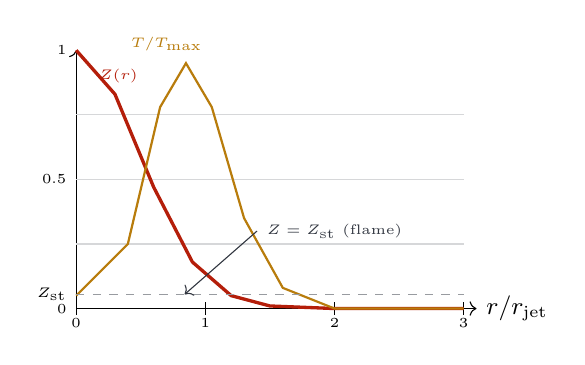
\begin{tikzpicture}[scale=0.82]
        % Axes
        \draw[->] (0,0) -- (6.2,0) node[right,font=\small]{$r/r_{\text{jet}}$};
        \draw[->] (0,0) -- (0,4.0) node[above,font=\small]{};
        % Y-tick labels
        \node[left,font=\tiny] at (0,0)   {0};
        \node[left,font=\tiny] at (0,0.22){$Z_{\text{st}}$};
        \node[left,font=\tiny] at (0,2.0) {0.5};
        \node[left,font=\tiny] at (0,4.0) {1};
        % X-tick labels
        \foreach \x/\lab in {0/0,2/1,4/2,6/3}{
          \draw (\x,-0.1)--(\x,0.1);
          \node[below,font=\tiny] at (\x,0) {\lab};
        }
        % Grid lines
        \foreach \y in {1,2,3}{
          \draw[ashgrey!20] (0,\y)--(6,\y);
        }
        % Z(r) profile - firered
        \draw[firered,very thick]
          (0,4.0)--(0.6,3.32)--(1.2,1.88)--(1.8,0.72)
          --(2.4,0.20)--(3.0,0.04)--(4.0,0)--(6.0,0);
        \node[firered,font=\tiny,right] at (0.2,3.6) {$Z(r)$};
        % T(r) profile - flameyellow bell
        \draw[flameyellow!80!black,thick]
          (0,0.2)--(0.8,1.0)--(1.3,3.12)--(1.7,3.80)
          --(2.1,3.12)--(2.6,1.40)--(3.2,0.32)--(4,0)--(6,0);
        \node[flameyellow!80!black,font=\tiny] at (1.4,4.1) {$T/T_{\max}$};
        % Stoichiometric line
        \draw[ashgrey!50,dashed] (0,0.22)--(6,0.22);
        % Stoich marker
        \draw[<-,ashgrey,thin] (1.68,0.22)--(2.8,1.2)
          node[right,font=\tiny,ashgrey]{$Z=\Zst$ (flame)};
      \end{tikzpicture}
    \end{column}
  \end{columns}
\end{frame}

\begin{frame}{Conserved Scalar: Why $Z$ Simplifies Everything}

  The transport equation for $Z$ (equal diffusivities, unity Le):
  \[
    \rho\pd{Z}{t} + \rho\mathbf{u}\cdot\nabla Z
    = \nabla\cdot(\rho D\nabla Z)
  \]
  \textbf{No source term} --- $Z$ is conserved regardless of whether
  reactions are occurring.

  \begin{columns}[t]
    \begin{column}{0.50\textwidth}
      \textbf{Flame-sheet (Burke--Schumann) limit}\\[3pt]
      Infinitely fast chemistry: all reactions are complete at $Z=\Zst$.
      Then temperature and species are \emph{functions of $Z$ alone}:
      \begin{align*}
        T &= T(Z)\\
        Y_F &= \max(0,\;Y_{F,1}(Z-\Zst)/(1-\Zst))\\
        Y_{\text{ox}} &= \max(0,\;Y_{\text{ox},2}(\Zst-Z)/\Zst)
      \end{align*}
      Fuel and oxidiser cannot coexist
      ($Y_F Y_{\text{ox}} = 0$ everywhere).
    \end{column}
    \begin{column}{0.46\textwidth}
      \textbf{Reducing complexity}
      \begin{itemize}
        \item 3-D reactive flow $\to$ solve \emph{one} scalar field $Z$
        \item Look up $T(Z)$, $Y_k(Z)$ from a
              chemistry library (flamelet)
        \item This is the basis of modern CFD
              \textbf{flamelet models} for turbulent non-premixed
              combustion
        \item Finite-rate effects are introduced via the scalar
              dissipation rate $\chi$ (next section)
      \end{itemize}
    \end{column}
  \end{columns}
\end{frame}

% =====================================================================
\section{Burke--Schumann Flame Structure}
% =====================================================================

\begin{frame}{The Burke--Schumann Solution}

  For the flame-sheet limit in a co-flowing round jet:
  the temperature and species profiles as functions of $Z$:

  \begin{center}
  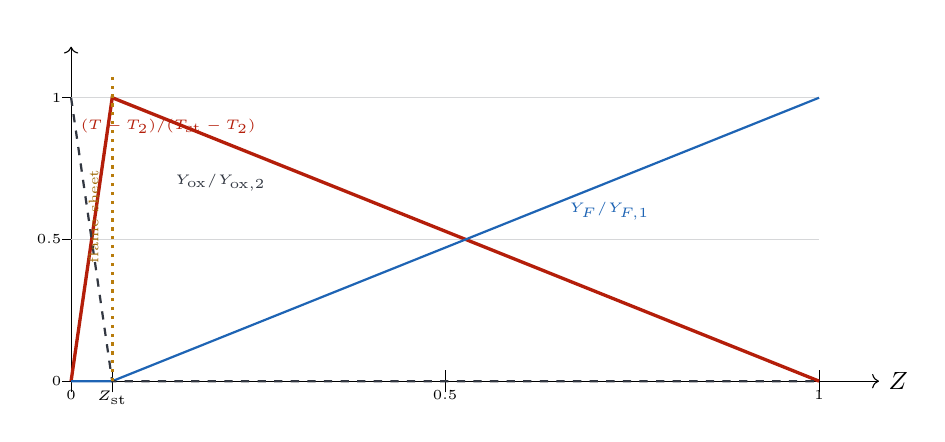
\begin{tikzpicture}[xscale=9.5, yscale=3.6]
    \draw[->] (0,0) -- (1.08,0) node[right,font=\small]{$Z$};
    \draw[->] (0,0) -- (0,1.18) node[above,font=\small]{};
    \foreach \x/\lab in {0/0, 0.055/$\Zst$, 0.5/0.5, 1.0/1}{
      \draw (\x,-0.04)--(\x,0.04);
      \node[below,font=\tiny] at (\x,0) {\lab};
    }
    \foreach \y/\lab in {0/0, 0.5/0.5, 1.0/1}{
      \draw (-0.012,\y)--(0.012,\y);
      \node[left,font=\tiny] at (0,\y) {\lab};
    }
    \draw[ashgrey!20] (0,0.5)--(1,0.5);
    \draw[ashgrey!20] (0,1.0)--(1,1.0);
    \draw[firered,very thick] (0,0)--(0.055,1.0)--(1.0,0);
    \node[firered,font=\tiny] at (0.13,0.9){$(T-T_2)/(T_{\text{st}}-T_2)$};
    \draw[skyblue,thick] (0,0)--(0.055,0)--(1.0,1.0);
    \node[skyblue,font=\tiny] at (0.72,0.60){$Y_F/Y_{F,1}$};
    \draw[ashgrey,thick,dashed] (0,1.0)--(0.055,0)--(1.0,0);
    \node[ashgrey,font=\tiny] at (0.20,0.70){$Y_{\text{ox}}/Y_{\text{ox},2}$};
    \draw[flameyellow!80!black,very thick,dotted]
      (0.055,0)--(0.055,1.08);
    \node[flameyellow!70!black,font=\tiny,rotate=90]
      at (0.030,0.58){flame sheet};
  \end{tikzpicture}
  \end{center}

  \small The flame temperature $\Tst$ is reached at $Z = \Zst$.
  Fuel and oxidiser profiles are piecewise linear and do not overlap.
\end{frame}

\begin{frame}{Scalar Dissipation Rate $\chi$ and Finite-Rate Effects}

  In reality chemistry is \textbf{not} infinitely fast.
  The key parameter controlling the departure from the flame-sheet
  limit is the \textbf{scalar dissipation rate}:
  \[
    \chi = 2D|\nabla Z|^2 \quad [\text{s}^{-1}]
  \]
  $\chi$ measures how fast mixture fraction gradients are smoothed out
  by diffusion --- i.e.\ how \emph{strained} the flame is.

  \begin{columns}[t]
    \begin{column}{0.50\textwidth}
      \textbf{Physical interpretation}
      \begin{itemize}
        \item High $\chi$: steep $Z$ gradients, fast mixing ---
              reactants are swept through the reaction zone before
              they can fully burn
        \item $1/\chi$ is the \emph{residence time} in the flame zone
        \item $\Da_{\text{flame}} \propto 1/(\chi\,\tchem)$:
              extinction when $\chi > \chiext$
      \end{itemize}
    \end{column}
    \begin{column}{0.46\textwidth}
      \begin{alertblock}{Extinction criterion}
        Flame extinction occurs when the scalar dissipation
        at the stoichiometric surface exceeds the critical value:
        \[
          \chist > \chiext \approx \frac{1}{\tchem(T_{\text{st}})}
        \]
        This is the \textbf{diffusion-flame blowout} condition ---
        the analogue of the WSR blowout from Unit~4.
      \end{alertblock}
    \end{column}
  \end{columns}
\end{frame}

\begin{frame}{The S-Curve for Diffusion Flames}

  Just as the WSR has an S-curve in $(T, \tau)$ space,
  the counterflow diffusion flame has an S-curve in
  $(T_{\text{st}}, \chi_{\text{st}})$ space:

  \begin{columns}
    \begin{column}{0.50\textwidth}
      \centering
      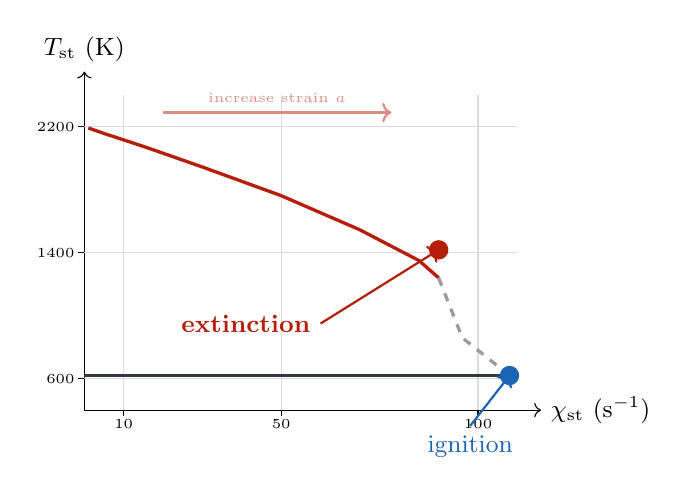
\begin{tikzpicture}[scale=1.0]
        \draw[->] (0,0) -- (5.8,0)
          node[right,font=\small]{$\chist$ (s$^{-1}$)};
        \draw[->] (0,0) -- (0,4.3)
          node[above,font=\small]{$T_{\text{st}}$ (K)};
        \draw (0.5,-0.08)--(0.5,0.08); \node[below,font=\tiny]at(0.5,0){10};
        \draw (2.5,-0.08)--(2.5,0.08); \node[below,font=\tiny]at(2.5,0){50};
        \draw (5.0,-0.08)--(5.0,0.08); \node[below,font=\tiny]at(5.0,0){100};
        \draw (-0.08,0.4)--(0.08,0.4); \node[left,font=\tiny]at(0,0.4){600};
        \draw (-0.08,2.0)--(0.08,2.0); \node[left,font=\tiny]at(0,2.0){1400};
        \draw (-0.08,3.6)--(0.08,3.6); \node[left,font=\tiny]at(0,3.6){2200};
        \draw[ashgrey!18](0,0.4)--(5.5,0.4);
        \draw[ashgrey!18](0,2.0)--(5.5,2.0);
        \draw[ashgrey!18](0,3.6)--(5.5,3.6);
        \draw[ashgrey!18](0.5,0)--(0.5,4.0);
        \draw[ashgrey!18](2.5,0)--(2.5,4.0);
        \draw[ashgrey!18](5.0,0)--(5.0,4.0);
        \draw[firered,very thick]
          (0.05,3.584) -- (0.25,3.514) --
          (0.75,3.35) -- (1.5,3.088) --
          (2.5,2.724) -- (3.5,2.29) --
          (4.25,1.9) -- (4.5,1.68);
        \draw[ashgrey,thick] (0,0.44) -- (5.5,0.44);
        \draw[ashgrey!50,dashed,very thick]
          (4.5,1.68) -- (4.8,0.92) --
          (5.1,0.68) -- (5.4,0.44);
        \fill[firered] (4.5,2.036) circle (3.5pt);
        \draw[<-,firered,thick]
          (4.5,2.036) -- (3.0,1.1)
          node[left,font=\small,firered]{\textbf{extinction}};
        \fill[skyblue] (5.4,0.44) circle (3.5pt);
        \draw[<-,skyblue,thick]
          (5.4,0.44) -- (4.9,-0.2)
          node[below,font=\small,skyblue]{ignition};
        \draw[->,firered!50,thick]
          (1.0,3.78) -- (3.9,3.78)
          node[midway,above,font=\tiny]{increase strain $a$};
      \end{tikzpicture}
    \end{column}
    \begin{column}{0.46\textwidth}
      \begin{itemize}
        \item \textbf{Upper branch}: burning flame; $T_{\text{st}}$
              decreases as $\chi_{\text{st}}$ increases (more strain
              $\to$ more heat loss $\to$ lower $T$)
        \item \textbf{Lower branch}: unignited (no flame)
        \item \textbf{Extinction point}: left turning point ---
              increasing $\chi$ past $\chiext$ causes abrupt
              extinction
        \item \textbf{Ignition point}: right turning point ---
              reducing $\chi$ from the cold branch causes jump
              to burning branch
        \item Key difference from WSR: $x$-axis is $\chi$ (mixing
              intensity), not $\taures$
      \end{itemize}
    \end{column}
  \end{columns}
\end{frame}

% =====================================================================
\section{Laminar Jet Diffusion Flames}
% =====================================================================

\begin{frame}{The Round Laminar Jet Flame: Roper's Correlation}

  The simplest diffusion flame: fuel issuing from a round tube into
  quiescent air.

  \begin{columns}
    \begin{column}{0.55\textwidth}
      \textbf{Flame height scaling (Roper 1977)}\\[3pt]
      For a laminar axisymmetric fuel jet:
      \[
        \Lf = \frac{Q_F}{4\pi D \ln(1 + 1/\Zst)}
      \]
      where $Q_F = u_F \pi r_j^2$ is the fuel volumetric flow rate
      and $D$ is the fuel--air diffusivity.

      Equivalently, in terms of the fuel velocity $u_F$:
      \[
        \Lf \propto \frac{r_j^2\,u_F}{D}
             = \frac{Q_F}{D}
      \]

      \begin{block}{Key result}
        Laminar flame height is proportional to \textbf{fuel flow rate}
        and \textbf{inversely proportional to diffusivity}.
        It is \emph{independent} of nozzle diameter for a fixed flow
        rate.
      \end{block}
    \end{column}
    \begin{column}{0.41\textwidth}
      \centering
      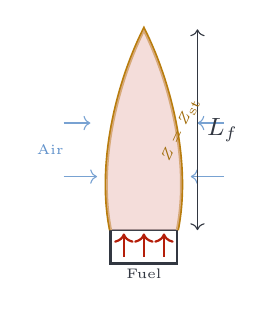
\begin{tikzpicture}[font=\small, scale=0.85]
        % Nozzle
        \draw[thick,ashgrey] (-0.5,-0.5) rectangle (0.5,0);
        % Flame outline
        \draw[very thick,flameyellow!80!black]
          (-0.5,0) .. controls (-0.7,1.0) and (-0.4,2.2) ..
          (0,3.0) .. controls (0.4,2.2) and (0.7,1.0) ..
          (0.5,0);
        \fill[firered!25,opacity=0.6]
          (-0.5,0) .. controls (-0.7,1.0) and (-0.4,2.2) ..
          (0,3.0) .. controls (0.4,2.2) and (0.7,1.0) ..
          (0.5,0) -- cycle;
        % Fuel arrows
        \foreach \x in {-0.3,0,0.3}{
          \draw[->,firered,thick] (\x,-0.4)--(\x,-0.05);
        }
        % Air diffusion arrows
        \draw[->,skyblue!60,thin] (-1.2,0.8)--(-0.7,0.8);
        \draw[->,skyblue!60,thin] (-1.2,1.6)--(-0.8,1.6);
        \draw[->,skyblue!60,thin] ( 1.2,0.8)--( 0.7,0.8);
        \draw[->,skyblue!60,thin] ( 1.2,1.6)--( 0.8,1.6);
        \node[skyblue!70,font=\tiny] at (-1.4,1.2){Air};
        % Height annotation
        \draw[<->,ashgrey,thin] (0.8,0)--(0.8,3.0)
          node[midway,right,font=\small]{$\Lf$};
        % Z=Zst surface
        \node[flameyellow!70!black,font=\tiny,rotate=65]
          at (0.55,1.5){$Z=\Zst$};
        \node[font=\tiny,ashgrey] at (0,-0.65){Fuel};
      \end{tikzpicture}
    \end{column}
  \end{columns}
\end{frame}

\begin{frame}{Laminar to Turbulent Transition in Jet Flames}

  \begin{columns}
    \begin{column}{0.55\textwidth}
      As fuel velocity $u_F$ increases:
      \begin{enumerate}
        \item \textbf{Laminar regime}: $\Lf \propto u_F$
              (Roper scaling)
        \item \textbf{Transition}: flame becomes unstable, tip flickers
        \item \textbf{Turbulent regime}: $\Lf \approx \text{const}$
              (independent of $u_F$!) ---
              turbulent diffusivity $D_t \propto u_F$, so
              $\Lf \sim Q_F/D_t \sim r_j^2 u_F / u_F \to r_j^2/\text{const}$
        \item \textbf{Liftoff}: the flame base detaches from the
              nozzle at a \textbf{liftoff height} $h_L$
        \item \textbf{Blowout}: at very high $u_F$ the flame is
              extinguished entirely
      \end{enumerate}
    \end{column}
    \begin{column}{0.41\textwidth}
      \centering
      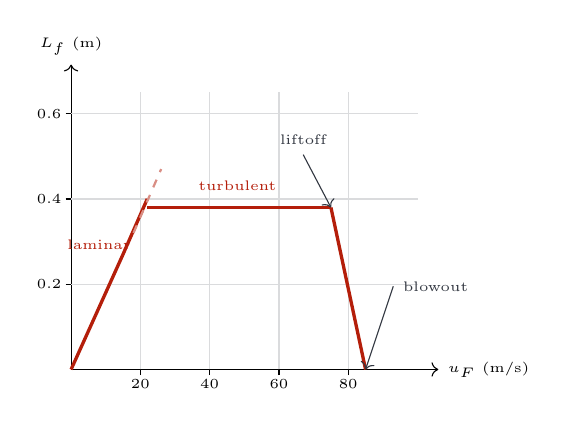
\begin{tikzpicture}[scale=0.88]
        \draw[->](0,0)--(5.3,0) node[right,font=\tiny]{$u_F$ (m/s)};
        \draw[->](0,0)--(0,4.4) node[above,font=\tiny]{$L_f$ (m)};
        \foreach \xx/\lab in {1.0/20,2.0/40,3.0/60,4.0/80}{
          \draw(\xx,-0.08)--(\xx,0.08);
          \node[below,font=\tiny]at(\xx,0){\lab};
        }
        \foreach \yy/\lab in {1.23/0.2,2.46/0.4,3.69/0.6}{
          \draw(-0.08,\yy)--(0.08,\yy);
          \node[left,font=\tiny]at(0,\yy){\lab};
        }
        \foreach \xx in {1.0,2.0,3.0,4.0}{\draw[ashgrey!18](\xx,0)--(\xx,4.0);}
        \foreach \yy in {1.23,2.46,3.69}{\draw[ashgrey!18](0,\yy)--(5.0,\yy);}
        \draw[firered,very thick]
          (0,0)--(0.25,0.554)--(0.5,1.108)--(0.75,1.662)--(1.1,2.462);
        \draw[firered,very thick]
          (1.1,2.338)--(3.0,2.338)--(3.75,2.338);
        \draw[firered!50,dashed,thick]
          (0.9,1.969)--(1.3,2.892);
        \draw[firered,very thick]
          (3.75,2.338)--(4.0,1.169)--(4.25,0);
        \node[firered,font=\tiny]at(0.4,1.8){laminar};
        \node[firered,font=\tiny]at(2.4,2.65){turbulent};
        \draw[<-,ashgrey,thin](3.75,2.338)--(3.35,3.1)
          node[above,font=\tiny]{liftoff};
        \draw[<-,ashgrey,thin](4.25,0)--(4.65,1.2)
          node[right,font=\tiny]{blowout};
      \end{tikzpicture}
    \end{column}
  \end{columns}
\end{frame}

% =====================================================================
\section{Counterflow Diffusion Flame}
% =====================================================================

\begin{frame}{The Counterflow Diffusion Flame}

  The \textbf{counterflow (opposed-jet) diffusion flame} is the
  canonical configuration for studying strain-rate effects.

  \begin{columns}
    \begin{column}{0.48\textwidth}
      \centering
      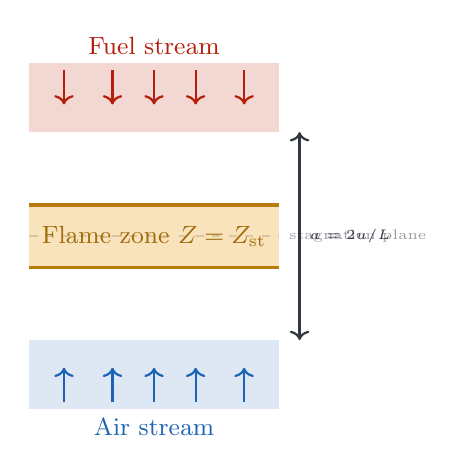
\begin{tikzpicture}[font=\small, scale=0.88]
        % Fuel jet (top, downward)
        \fill[firered!18] (-1.8,1.5) rectangle (1.8,2.5);
        \foreach \x in {-1.3,-0.6,0,0.6,1.3}{
          \draw[->,firered,thick] (\x,2.4)--(\x,1.9);
        }
        \node[firered,font=\small] at (0,2.75) {Fuel stream};

        % Air jet (bottom, upward)
        \fill[skyblue!15] (-1.8,-2.5) rectangle (1.8,-1.5);
        \foreach \x in {-1.3,-0.6,0,0.6,1.3}{
          \draw[->,skyblue,thick] (\x,-2.4)--(\x,-1.9);
        }
        \node[skyblue,font=\small] at (0,-2.75) {Air stream};

        % Stagnation plane
        \draw[ashgrey!50,dashed,thick] (-1.8,0)--(1.8,0)
          node[right,font=\tiny]{stagnation plane};

        % Flame sheet (slightly below stagnation for fuel side)
        \fill[flameyellow!40,opacity=0.7]
          (-1.8,-0.45) rectangle (1.8,0.45);
        \draw[flameyellow!80!black,very thick]
          (-1.8,-0.45)--(1.8,-0.45);
        \draw[flameyellow!80!black,very thick]
          (-1.8, 0.45)--(1.8, 0.45);
        \node[flameyellow!70!black,font=\small]
          at (0,0) {Flame zone $Z=\Zst$};

        % Strain rate annotation
        \draw[<->,thick,ashgrey] (2.1,-1.5)--(2.1,1.5)
          node[midway,right,font=\tiny]{$a = 2u/L$};
      \end{tikzpicture}
    \end{column}
    \begin{column}{0.48\textwidth}
      \textbf{Strain rate} $a$ (s$^{-1}$):
      \[
        a = \frac{2 u_{\text{ox}}}{L}
          \left(1 + \frac{u_F\sqrt{\rho_F}}{u_{\text{ox}}\sqrt{\rho_{\text{ox}}}}\right)
      \]
      \begin{itemize}
        \item Controls the scalar dissipation at the stoichiometric
              surface: $\chist \propto a\,e^{-2[\text{erfinv}(\Zst)]^2}$
        \item Laboratory workhorse for measuring
              \textbf{extinction strain rates} $a_{\text{ext}}$
        \item Used to build \textbf{flamelet libraries}:
              tabulate $(T, Y_k)$ as functions of $(Z, \chi)$
              over the full range from equilibrium to extinction
        \item Direct input to CFD turbulent combustion models
      \end{itemize}
    \end{column}
  \end{columns}
\end{frame}

\begin{frame}{Flamelet Concept: Chemistry Parameterised by $Z$ and $\chi$}

  \begin{block}{Flamelet model}
    In a turbulent non-premixed flame, the local reaction zone is
    thin compared to turbulent length scales.
    It behaves locally as a \textbf{laminar diffusion flame}
    (flamelet) embedded in a turbulent flow.
    The thermo-chemistry is fully described by:
    \[
      \phi = \phi(Z,\,\chi)
    \]
  \end{block}

  \begin{columns}[t]
    \begin{column}{0.50\textwidth}
      \textbf{Steady flamelet equations}
      \[
        \rho\frac{\partial Y_k}{\partial t}
        = \frac{\rho\chi}{2}\frac{\partial^2 Y_k}{\partial Z^2}
          + \wdot_k W_k
      \]
      \[
        \rho\frac{\partial T}{\partial t}
        = \frac{\rho\chi}{2}\frac{\partial^2 T}{\partial Z^2}
          - \frac{1}{c_p}\sum_k h_k\wdot_k W_k
      \]
      Solved as a 1-D problem in $Z$-space for each $\chi$.
    \end{column}
    \begin{column}{0.46\textwidth}
      \textbf{Workflow in turbulent CFD}
      \begin{enumerate}
        \item Pre-compute flamelet library
              $\{T,\,Y_k\}(Z,\,\chi)$ offline
        \item CFD solves for $\tilde{Z}$,
              $\widetilde{Z''^2}$, $\tilde{\chi}$
        \item Retrieve $\tilde{T}$, $\tilde{Y}_k$
              by table look-up
        \item $\mathcal{O}(10\times)$ cheaper than
              transporting all species in CFD
      \end{enumerate}
    \end{column}
  \end{columns}
\end{frame}

% =====================================================================
\section{Soot and NO\texorpdfstring{$_x$}{x} Formation}
% =====================================================================

\begin{frame}{Soot Formation in Diffusion Flames}

  Soot forms on the \textbf{rich side} of a diffusion flame
  ($Z > \Zst$) where carbon-rich pyrolysis products accumulate.

  \begin{columns}[t]
    \begin{column}{0.54\textwidth}
      \textbf{Soot inception pathway}
      \begin{enumerate}
        \item Fuel pyrolysis: \ch{CH4} $\to$ \ch{C2H2}
              (acetylene), \ch{C2H4}, PAH
        \item \textbf{HACA mechanism}: H-abstraction + C$_2$H$_2$
              addition grows PAH (poly-cyclic aromatic hydrocarbons)
        \item Soot particle inception from PAH
        \item Surface growth, coagulation, agglomeration
        \item Oxidation by O, OH, O$_2$ on the fuel-lean side
      \end{enumerate}
    \end{column}
    \begin{column}{0.42\textwidth}
      \begin{alertblock}{Aeronautical impact}
        Soot (black carbon) from aviation:
        \begin{itemize}
          \item PM$_{2.5}$ health impact near airports
          \item Contrail ice nucleation --- climate forcing
          \item Reduced combustor life via liner deposition
          \item ICAO Annex~16 non-volatile PM regulations
                tightening from 2023
        \end{itemize}
        Controlled by reducing the rich primary zone
        (RQL $\to$ LPP transition).
      \end{alertblock}
    \end{column}
  \end{columns}

  \begin{exampleblock}{Mixing fraction criterion}
    Soot forms where $Z > \Zst$ and $T > T_{\text{soot,onset}}
    \approx 1300$~K.
    Suppression requires reducing the rich-side residence time ---
    exactly the motivation for the quick-quench in RQL combustors.
  \end{exampleblock}
\end{frame}

\begin{frame}{NO$_x$ Formation in Diffusion Flames}

  NO formation mechanisms differ on each side of the flame:

  \vspace{3pt}
  \begin{center}
  \renewcommand{\arraystretch}{1.35}
  \begin{tabular}{>{\bfseries}p{2.8cm} p{4.3cm} p{4.5cm}}
    \toprule
    Mechanism & Location & Key driver \\
    \midrule
    Thermal (Zeldovich) & $Z < \Zst$ (lean side) near flame &
      Very high $T_{\text{st}}$ ($> 1800$~K);
      rate $\propto e^{-38000/T}$ \\
    Prompt (Fenimore) & $Z > \Zst$ (rich side) &
      CH radical reacts with N$_2$:
      $\text{CH} + \text{N}_2 \to \text{HCN} + \text{N}$ \\
    Fuel-bound N & Anywhere & N atoms in fuel (Jet-A
      $< 0.1$\% N; coal much higher) \\
    N$_2$O pathway & Lean, high-$p$ & Important in
      lean-premixed burners at high pressure \\
    \bottomrule
  \end{tabular}
  \end{center}

  \begin{block}{Design strategy}
    Reducing $T_{\text{st}}$ (via leaner $\Zst$ or dilution)
    exponentially cuts thermal NO.
    The RQL combustor quenches the flame before thermal NO
    can accumulate; LPP avoids high $T_{\text{st}}$ entirely.
  \end{block}
\end{frame}

% =====================================================================
\section{Liftoff and Blowout}
% =====================================================================

\begin{frame}{Liftoff: Flame Detachment from the Nozzle}

  At sufficiently high fuel velocity, the flame base detaches and
  \textbf{lifts off} to a height $h_L$ above the nozzle.

  \begin{columns}[t]
    \begin{column}{0.55\textwidth}
      \textbf{Physical mechanism (Peters--Williams model)}
      \begin{itemize}
        \item At the flame base, the local flow velocity $u$
              must equal the \textbf{local premixed flame speed}
              $\SL$ of the partially premixed mixture
        \item Liftoff height is where this balance is achieved:
              \[
                u(h_L,r_{\text{st}}) = \SL(Z_{\text{near st}})
              \]
        \item As $u_F \uparrow$: balance point moves downstream
              $\Rightarrow$ $h_L \uparrow$
        \item Liftoff height scales as:
              \[
                h_L \propto \frac{u_F^3}{S_{L,\max}^2}
                \left(\frac{D}{\nu}\right)
              \]
      \end{itemize}
    \end{column}
    \begin{column}{0.41\textwidth}
      \begin{exampleblock}{Key point}
        Liftoff is a \textbf{premixed-flame phenomenon}:
        the leading edge of a lifted diffusion flame is a
        tribrachial (triple) flame with premixed wings
        and a non-premixed trailing edge.
        This links diffusion flame stability directly to the
        premixed burning velocity $\SL$ from Unit~6.
      \end{exampleblock}
      \vspace{4pt}
      \begin{alertblock}{Blowout}
        When $h_L \to \infty$, the flame is blown out.
        Critical condition:
        $\Da_{\text{liftoff}} = \SL^2\,h_L/(D\,u_F) < \Da_{\text{crit}}$
      \end{alertblock}
    \end{column}
  \end{columns}
\end{frame}

% =====================================================================
\section{Turbulent Diffusion Flames and Aero Applications}
% =====================================================================

\begin{frame}{Turbulent Diffusion Flames: Key Differences}

  Practical aero-engine diffusion flames are almost always turbulent.

  \begin{columns}[t]
    \begin{column}{0.50\textwidth}
      \textbf{Effect of turbulence}
      \begin{itemize}
        \item Turbulent eddies wrinkle the flame surface ---
              greatly increase the \emph{stoichiometric surface area}
        \item Turbulent scalar dissipation
              $\tilde{\chi}_{\text{st}}$ fluctuates in time;
              local extinction events occur when
              $\chi_{\text{st}} > \chiext$
        \item Turbulent mixing time replaces molecular $D$:
              $D_t \sim k^2/\epsilon$
        \item Turbulent flame height $\Lf \approx \text{const}$
              (independent of $u_F$ --- confirmed experimentally)
      \end{itemize}
    \end{column}
    \begin{column}{0.46\textwidth}
      \textbf{Turbulent jet flame height}
      \[
        \Lf \approx C\,r_j \cdot
        \frac{\sqrt{\rho_F/\rho_{\text{air}}}}{\Zst}
      \]
      where $C \approx 5.3$ (Hawthorne et al.\ 1949).

      \vspace{4pt}
      \begin{itemize}
        \item Depends on nozzle radius $r_j$ and
              stoichiometric mixture fraction $\Zst$
        \item Independent of $u_F$ once fully turbulent
        \item Shorter for fuels with high $\Zst$
              (H$_2$: $\Zst \approx 0.028$, very short flame)
      \end{itemize}
    \end{column}
  \end{columns}
\end{frame}

\begin{frame}{Gas Turbine Combustor: Diffusion Flame Physics}

  \begin{center}
  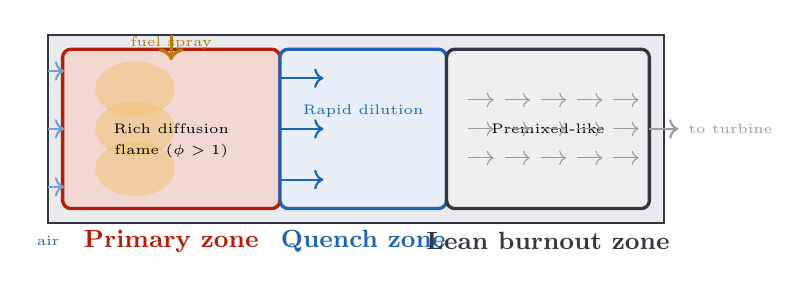
\begin{tikzpicture}[font=\small, scale=0.92]
    % Combustor liner
    \draw[thick,ashgrey,fill=ashgrey!10]
      (0,1.3) -- (8.5,1.3) -- (8.5,-1.3) -- (0,-1.3) -- cycle;

    % Primary zone (rich, diffusion flame)
    \draw[very thick,firered,fill=firered!18,rounded corners=3pt]
      (0.2,1.1) rectangle (3.2,-1.1);
    \foreach \cy in {0.55, 0.0, -0.55}{
      \fill[flameyellow!60,opacity=0.5]
        (1.2,\cy) ellipse (0.55 and 0.38);
    }
    \node[firered,font=\small\bfseries] at (1.7,-1.55)
      {Primary zone};
    \node[font=\tiny] at (1.7,0) {Rich diffusion};
    \node[font=\tiny] at (1.7,-0.3) {flame ($\phi>1$)};

    % Dilution/quench zone
    \draw[very thick,skyblue,fill=skyblue!10,rounded corners=3pt]
      (3.2,1.1) rectangle (5.5,-1.1);
    \foreach \y in {0.7,0.0,-0.7}{
      \draw[->,skyblue,thick] (3.2,\y)--(3.8,\y);
    }
    \node[skyblue,font=\small\bfseries] at (4.35,-1.55)
      {Quench zone};
    \node[font=\tiny,skyblue] at (4.35,0.25) {Rapid dilution};

    % Lean zone
    \draw[very thick,ashgrey,fill=ashgrey!8,rounded corners=3pt]
      (5.5,1.1) rectangle (8.3,-1.1);
    \node[ashgrey,font=\small\bfseries] at (6.9,-1.55)
      {Lean burnout zone};
    \node[font=\tiny] at (6.9,0) {Premixed-like};
    \foreach \xx in {5.8,6.3,6.8,7.3,7.8}{
      \draw[->,ashgrey!50,thin] (\xx,0.4)--(\xx+0.35,0.4);
      \draw[->,ashgrey!50,thin] (\xx,0.0)--(\xx+0.35,0.0);
      \draw[->,ashgrey!50,thin] (\xx,-0.4)--(\xx+0.35,-0.4);
    }

    % Fuel injector arrow
    \draw[->,flameyellow!80!black,very thick]
      (1.7,1.3)--(1.7,0.95)
      node[above,font=\tiny,flameyellow!80!black]{fuel spray};

    % Labels
    \node[font=\tiny,skyblue] at (0,-1.55) {air};
    \draw[->,skyblue!60,thick] (0,0.8)--(0.22,0.8);
    \draw[->,skyblue!60,thick] (0,0.0)--(0.22,0.0);
    \draw[->,skyblue!60,thick] (0,-0.8)--(0.22,-0.8);
    \draw[->,ashgrey!50,thick] (8.3,0)--(8.7,0)
      node[right,font=\tiny]{to turbine};
  \end{tikzpicture}
  \end{center}

  \begin{itemize}
    \item \textbf{Primary zone}: turbulent diffusion flame around
          fuel spray; $Z > \Zst$; soot formation occurs here
    \item \textbf{Quench zone}: dilution air collapses the stoichiometric
          surface; rapid quench of rich products
    \item \textbf{Lean burnout}: WSR--PFR series behaviour
          (Units~4--5); CO and soot oxidised
  \end{itemize}
\end{frame}

\begin{frame}{Rocket Combustion: Diffusion Flame at Extremes}

  Rocket thrust chambers operate diffusion flames at conditions
  far beyond any gas turbine:

  \begin{columns}[t]
    \begin{column}{0.50\textwidth}
      \textbf{LOX/LH$_2$ coaxial injector element}
      \begin{itemize}
        \item Liquid oxygen (inner) + gaseous H$_2$ (outer annulus)
        \item Vaporisation, mixing, and combustion in $\sim$1 ms
        \item $p \sim 10$--$20$ MPa (100--200 bar)
        \item $T_{\text{st}} \approx 3600$ K
        \item $\Zst \approx 0.11$ (H$_2$/O$_2$)
        \item Flame height $\Lf \sim 5$--$20$ mm per injector
              element --- many hundreds of elements per chamber
      \end{itemize}
    \end{column}
    \begin{column}{0.46\textwidth}
      \begin{alertblock}{Extreme conditions}
        At 200 bar and 3600 K, the assumption of ideal gas and
        unity Lewis number both break down.
        Real-fluid (supercritical) thermodynamics are required.
        The ``flame'' is a thin region of sharp density gradient
        between cryogenic oxygen and hot products.
      \end{alertblock}
      \vspace{3pt}
      \begin{exampleblock}{Mixture fraction still applies}
        Even at supercritical conditions, $Z$ remains a
        well-defined conserved scalar and the flamelet
        framework is used for rocket injector CFD.
      \end{exampleblock}
    \end{column}
  \end{columns}
\end{frame}

% =====================================================================
\section{Summary}
% =====================================================================

\begin{frame}{Key Equations at a Glance}
  \renewcommand{\arraystretch}{1.6}
  \begin{tabular}{>{\bfseries}p{4.0cm} p{7.5cm}}
    \toprule
    Concept & Expression \\
    \midrule
    Mixture fraction & $Z \in [0,1]$; flame at $Z = \Zst$ \\
    Stoichiometric $Z$ & $\Zst = 1/(1 + sY_{F,1}/Y_{\text{ox},2})$ \\
    Conserved scalar & $\rho DZ/Dt = \nabla\cdot(\rho D\nabla Z)$ ---
                       no source term \\
    Scalar dissipation & $\chi = 2D|\nabla Z|^2$; extinction when
                         $\chist > \chiext$ \\
    Laminar flame height & $\Lf \propto Q_F/D$
                           (Roper; independent of $r_j$) \\
    Turbulent flame height &
      $\Lf \approx 5.3\,r_j\sqrt{\rho_F/\rho_{\text{air}}}/\Zst$ ---
      independent of $u_F$ \\
    Liftoff condition & $u(h_L) = \SL$
                        (premixed-flame balance at base) \\
    Flamelet & $T,Y_k = f(Z,\chi)$ --- 1-D chemistry in $Z$-space \\
    \bottomrule
  \end{tabular}
\end{frame}

\begin{frame}{Summary \& Take-Away Points}
  \begin{itemize}
    \item Diffusion flames are controlled by \textbf{mixing}, not
          chemistry; the flame sits on the stoichiometric surface
          $Z = \Zst$.
    \item The \textbf{mixture fraction} $Z$ is a conserved scalar
          with no source term --- it is the master variable for
          non-premixed combustion.
    \item \textbf{Infinite-rate chemistry} (Burke--Schumann): species
          and temperature are piecewise linear in $Z$; fuel and
          oxidiser cannot coexist.
    \item \textbf{Finite-rate effects} are captured by the scalar
          dissipation rate $\chi$; extinction occurs when
          $\chist > \chiext$, analogous to WSR blowout.
    \item Laminar jet flame height scales as $\Lf \propto Q_F/D$;
          turbulent flame height is \emph{independent of} $u_F$.
    \item \textbf{Soot} forms on the rich side ($Z > \Zst$, $T > 1300$ K);
          \textbf{thermal NO} forms on the lean side near the flame sheet.
    \item Liftoff and blowout are governed by the balance between
          local flow velocity and the premixed burning velocity
          $\SL$ at the flame base --- linking diffusion and premixed
          flame physics.
  \end{itemize}
  \vfill
  \begin{center}
    \large\textbf{Next lecture:} Turbulent Premixed Flames
    \& Combustion Regime Diagrams
  \end{center}
\end{frame}

% -- Closing slide ----------------------------------------------------
{
\setbeamertemplate{footline}{}
\setbeamertemplate{headline}{}
\setbeamercolor{background canvas}{bg=ashgrey}
\begin{frame}[plain, c]

  \begin{tikzpicture}[remember picture, overlay]
    \fill[ashgrey]
      (current page.south west) rectangle (current page.north east);
    \fill[firered, opacity=0.15]
      (current page.south east) circle (4.5cm);
    \fill[flameyellow, opacity=0.08]
      (current page.south east) circle (2.5cm);
  \end{tikzpicture}

  \vspace{0.55cm}
  {\color{white}\fontsize{22}{26}\selectfont\bfseries
   Diffusion Flames}

  \vspace{0.10cm}
  {\color{skyblue!70}\fontsize{9}{11}\selectfont
   Unit 7\enspace|\enspace
   Propulsion \& Combustion\enspace|\enspace
   Aeronautical Engineering Yr\,4}

  \vspace{0.12cm}
  
\begin{tikzpicture}
    \draw[skyblue!60, line width=0.6pt] (0,0) -- (\textwidth,0);
    \draw[firered, line width=2.2pt] (0,0) -- (0.28\textwidth,0);
  \end{tikzpicture}

  \vspace{0.30cm}

  \begin{columns}[t, totalwidth=\textwidth]
    \begin{column}{0.315\textwidth}
      \begin{beamercolorbox}[rounded=true,wd=\linewidth,
                             sep=6pt,center]{block title}
        \textbf{\small Mixing-Controlled Physics}
      \end{beamercolorbox}
      \vspace{3pt}
      \begin{beamercolorbox}[rounded=true,wd=\linewidth,
                             sep=6pt,center]{block body}
        \color{ashgrey}\fontsize{7.5}{10}\selectfont
        Mixture fraction $Z$: conserved scalar\\[3pt]
        Flame at $Z = Z_{\text{st}}$\\[3pt]
        Burke--Schumann flame-sheet limit\\[3pt]
        Scalar dissipation $\chi = 2D|\nabla Z|^2$
      \end{beamercolorbox}
    \end{column}
    \hfill
    \begin{column}{0.315\textwidth}
      \begin{beamercolorbox}[rounded=true,wd=\linewidth,
                             sep=6pt,center]{block title alerted}
        \textbf{\small Extinction \& Liftoff}
      \end{beamercolorbox}
      \vspace{3pt}
      \begin{beamercolorbox}[rounded=true,wd=\linewidth,
                             sep=6pt,center]{block body alerted}
        \color{ashgrey}\fontsize{7.5}{10}\selectfont
        $\chi_{\text{st}} > \chi_{\text{ext}}$: extinction\\[3pt]
        Liftoff: $u(h_L) = S_L$ (triple flame)\\[3pt]
        Turbulent $L_f$ independent of $u_F$\\[3pt]
        Flamelet: $T,Y_k = f(Z,\chi)$
      \end{beamercolorbox}
    \end{column}
    \hfill
    \begin{column}{0.315\textwidth}
      \begin{beamercolorbox}[rounded=true,wd=\linewidth,
                             sep=6pt,center]{block title example}
        \textbf{\small Propulsion Context}
      \end{beamercolorbox}
      \vspace{3pt}
      \begin{beamercolorbox}[rounded=true,wd=\linewidth,
                             sep=6pt,center]{block body example}
        \color{white}\fontsize{7.5}{10}\selectfont
        Gas turbine: RQL primary zone\\[3pt]
        Rocket: LOX/LH$_2$ coaxial injector\\[3pt]
        Soot formation on rich side\\[3pt]
        Thermal NO on lean side near flame
      \end{beamercolorbox}
    \end{column}
  \end{columns}

  \vspace{0.30cm}

  \begin{beamercolorbox}[rounded=true,wd=\textwidth,
                         sep=5pt,center]{block body}
    \color{skyblue!80}\fontsize{7.8}{10}\selectfont
    $Z_{\text{st}} = 1/(1+sY_{F,1}/Y_{\text{ox},2})$
    \quad\vrule width 0.4pt height 9pt depth 2pt\quad
    $\chi = 2D|\nabla Z|^2$
    \quad\vrule width 0.4pt height 9pt depth 2pt\quad
    $L_f \propto Q_F/D$
    \quad\vrule width 0.4pt height 9pt depth 2pt\quad
    $L_f^{\text{turb}} \approx 5.3\,r_j\sqrt{\rho_F/\rho_{\text{air}}}/Z_{\text{st}}$
  \end{beamercolorbox}

  \vspace{0.22cm}
  \begin{center}
    {\color{white!50}\fontsize{7.5}{9}\selectfont
     \textbf{Next:}\enspace
     Unit 8 --- Turbulent Premixed Flames \& Combustion Regime Diagrams}
  \end{center}
\end{frame}
}

% =====================================================================
\appendix
\begin{frame}{Practice Problems}
  \begin{enumerate}
    \item For a methane--air diffusion flame ($Y_{F,1}=1$,
          $Y_{\text{ox},2}=0.233$), calculate $\Zst$ and the
          stoichiometric temperature using $\Tad = T_2
          + \Zst Q_{\text{HV}} Y_{F,1}/c_p$
          with $T_2 = 300$~K, $Q_{\text{HV}} = 50$ MJ/kg,
          $c_p = 1.1$ kJ/(kg$\cdot$K).
          Explain physically why $\Zst$ is much less than 0.5.

    \item A laminar CH$_4$--air jet flame burns at $Q_F =
          3\times10^{-6}$ m$^3$/s with $D = 2\times10^{-5}$ m$^2$/s.
          Estimate the flame height using Roper's formula.
          If the fuel flow rate is doubled, what happens to $\Lf$?
          What happens when the flame becomes turbulent?

    \item Explain the physical meaning of the scalar dissipation
          rate $\chi$ and describe what happens to the flame temperature
          $T_{\text{st}}$ as $\chi_{\text{st}}$ is increased from
          zero to $\chi_{\text{ext}}$.
          How does this relate to the WSR S-curve from Unit~4?

    \item A gas turbine designer is choosing between an RQL and an LPP
          combustor for a new engine.
          Using the concepts of mixture fraction, scalar dissipation,
          and soot formation, outline the key trade-offs between the
          two designs in terms of: (a) NO$_x$ emissions, (b) soot/PM,
          (c) combustion stability, and (d) flashback risk.
  \end{enumerate}
\end{frame}

\end{document}
